\chapter{SystemCalls \& Permessi}

\section{System Calls}

In linux le applicazioni vengono eseguite nel cosiddetto \textit{user space},
uno spazio che ha un minor numero di permessi rispetto al kernel del sistema.
Se un'applicazione però vuole effettuare operazioni come accedere ad un file
o comunicare tramite la rete deve per forza comunicare tali azioni al kernel.
Nella programmazione, per effettuare queste azioni esistono delle interfacce
chiamate \textbf{systemcall}. Alcuni esempi di systemcall sono:

\begin{itemize}
    \item \verb|read|
    \item \verb|write|
    \item \verb|open|
    \item \verb|execve|
    \item \verb|chown|
    \item \verb|clone|
\end{itemize}

Solitamente i programmi hanno interfacce a più alto livello che gestiscono queste
systemcall ed i programmatori non devono preoccuparsene. I livelli di astrazione
più bassi che si utilizzano di solito sono \verb|glibc| e il pacchetto
\verb|syscall| per Golang.

\section{File Permissions}

Un aspetto molto importante in linux riguarda i permessi dei file, dato che in
linux tutto quanto è un file, anche dispositivi fisici come stampanti e schermi.
È facilmente comprensibile perché è di vitale importanza fornire i permessi per
la modifica dei file. Questi permessi vengono anche chiamati DAC:
\textit{Discretionatory Access Control}.\\

È possibile vedere la lista di file in una directory con i relativi permessi
eseguendo il comando:

\begin{lstlisting}[language=Bash]
    ls -l
\end{lstlisting}

\begin{figure}[H]
    \centering
    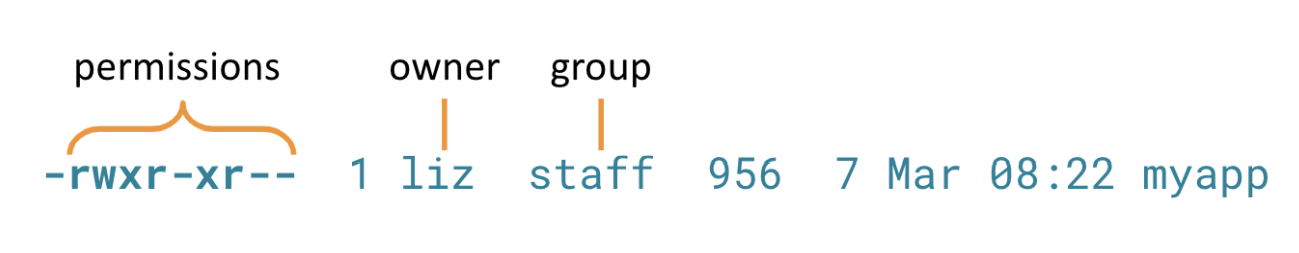
\includegraphics[width=10cm, keepaspectratio]{capitoli/os_security/imgs/permessi.png}
    \caption{Esempio di output del comando ls -l.}
\end{figure}

I permessi sono identificati con 9 simboli (si esclude il primo che rappresenta
se il file in questione è una directory) che possono essere visti come suddivisi
in gruppi di 3:

\begin{itemize}
    \item Il \textbf{primo} gruppo descrive i permessi dell'utente che possiede il file,
    \item Il \textbf{secondo} gruppo descrive i permessi del gruppo a cui appartiene il file,
    \item Il \textbf{terzo} descrive i permessi di tutti gli altri utenti.
\end{itemize}

Questi simboli corrispondono ad un bit che può essere o meno settato. In particolare
nell'immagine possiamo vedere i seguenti simboli:

\begin{itemize}
    \item \textit{r} (read)
    \item \textit{w} (write)
    \item \textit{x} (execute)
\end{itemize}

\subsection{setuid}

Normalmente, quando l'esecuzione di un file inizia, il processo che verrà creato
erediterà l'ID dell'utente che lo ha avviato. Tuttavia, se viene settato uno speciale
bit chiamato \textit{setuid}, il processo avrà lo stesso ID del proprietario
del file (owner) e non di chi lo ha avviato.\\

Nell'esempio sotto, possiamo vedere che copiando il file eseguibile \verb|sleep|
il proprietario ed il gruppo del file cambieranno diventando quelli dell'utente
(non-root user).

%%TODO: vedere se riscrivere le foto in testo

\begin{figure}[H]
    \centering
    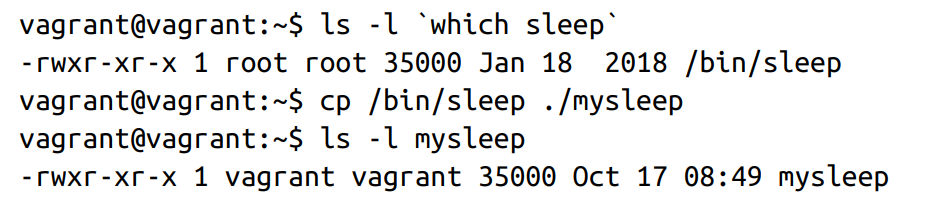
\includegraphics[width=\textwidth, keepaspectratio]{capitoli/os_security/imgs/setuid1.png}
\end{figure}

Eseguendolo come root e osservando i processi in esecuzione, possiamo notare che,
sia il processo \verb|sudo| che \verb|mysleep| hanno come \verb|UID| 0, che è quello
dell'utente root.

\begin{figure}[H]
    \centering
    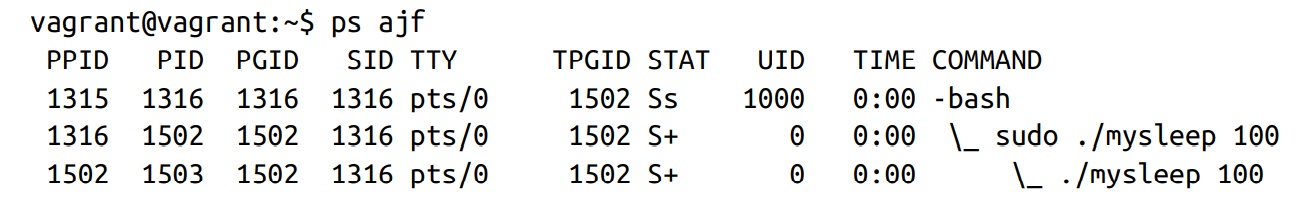
\includegraphics[width=\textwidth, keepaspectratio]{capitoli/os_security/imgs/setuid2.png}
\end{figure}


Ora abiliteremo il bit \textit{setuid}.

\begin{figure}[H]
    \centering
    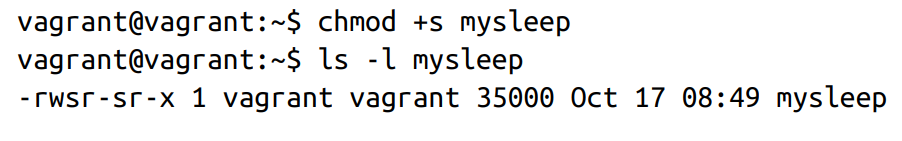
\includegraphics[width=\textwidth, keepaspectratio]{capitoli/os_security/imgs/setuid3.png}
\end{figure}

Possiamo vedere dove prima c'era \textit{x} per la parte di permessi del gruppo e
del proprietario, ora c'è \textit{s}. Proviamo a riavviare il processo \verb|mysleep|
e osserviamo i processi in esecuzione:

\begin{figure}[H]
    \centering
    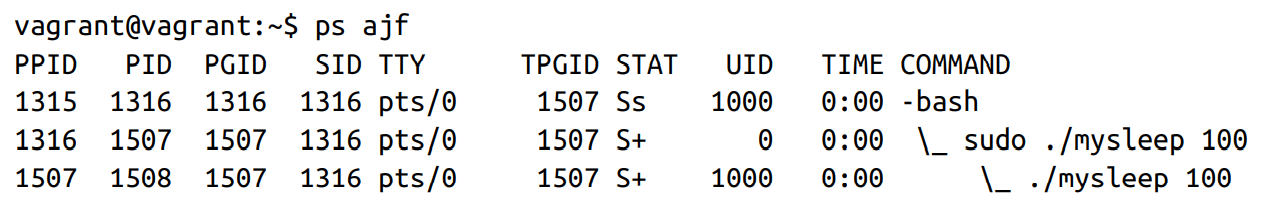
\includegraphics[width=\textwidth, keepaspectratio]{capitoli/os_security/imgs/setuid4.png}
\end{figure}

Possiamo vedere che il processo \verb|sudo| viene eseguito come root ma il processo
mysleep ha lo UID del proprietario del file (1000).\\

Questo bit viene tipicamente usato per dare ad un programma privilegi di cui ha
bisogno ma che non sono forniti agli utenti regolari. L'esempio pratico più comune
è quello del comando \verb|ping|, che necessita di speciali permessi per aprire
dei \textit{raw network socket}. \verb|ping| viene spesso installato con il bit
\textit{setuid} settato ed essendo di proprietà di root potrà essere eseguito con
i privilegi associati all'utente root (senza la necessità di sudo).\\
Per testare questo comportamento proviamo a copiare l'eseguibile di \verb|ping|
in modo da cambiare il proprietario e il gruppo ad un non-root user.

\begin{figure}[H]
    \centering
    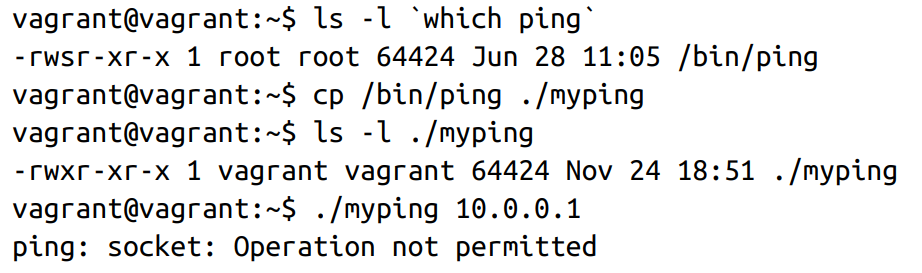
\includegraphics[width=\textwidth, keepaspectratio]{capitoli/os_security/imgs/ping1.png}
\end{figure}

Come possiamo vedere dall'esempio, il comando non va a buon fine perché durante
l'operazione di copia il bit \textit{setuid} non viene mantenuto.\\

Proviamo ora a cambiare il proprietario del file in root e possiamo notare che
l'esecuzione non va comunque a buon fine (adesso avremmo bisogno di sudo per farlo partire):

\begin{figure}[H]
    \centering
    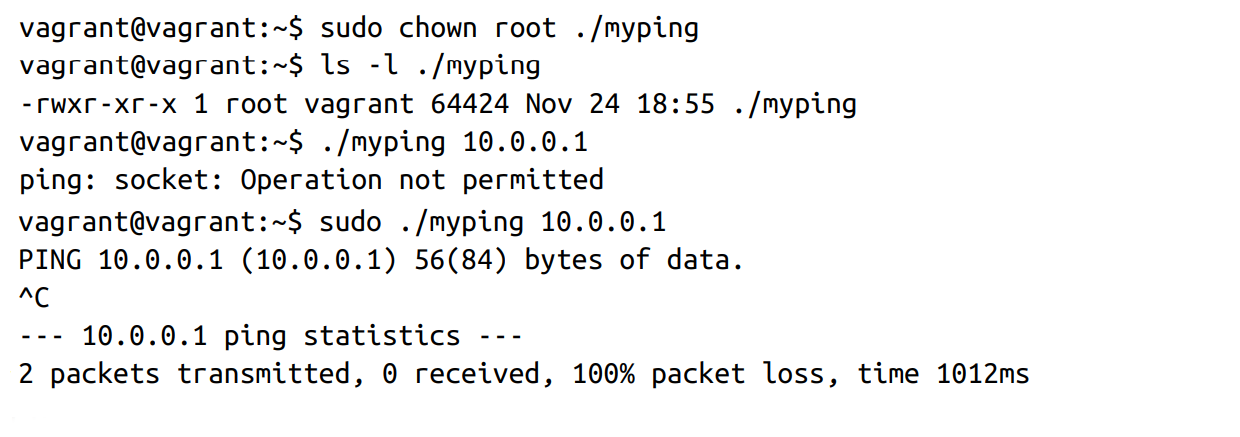
\includegraphics[width=\textwidth, keepaspectratio]{capitoli/os_security/imgs/ping2.png}
\end{figure}

Infine proviamo a settare il bit \textit{setuid} e riproviamo:

\begin{figure}[H]
    \centering
    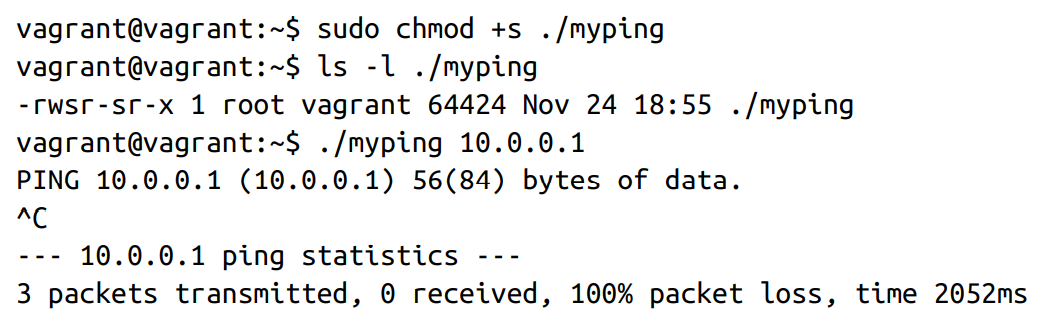
\includegraphics[width=\textwidth, keepaspectratio]{capitoli/os_security/imgs/ping3.png}
\end{figure}

Andando a vedere ora i processi in esecuzione, ci aspetteremmo che il processo myping
venga eseguito con UID 0 (root) ma non è questo il caso.

\begin{figure}[H]
    \centering
    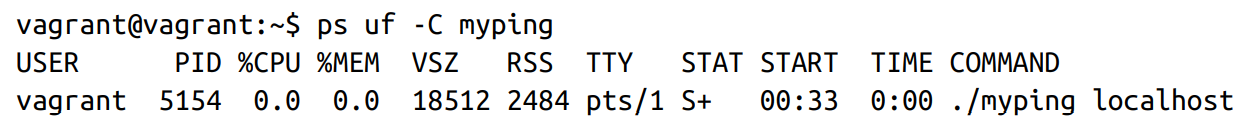
\includegraphics[width=\textwidth, keepaspectratio]{capitoli/os_security/imgs/ping4.png}
\end{figure}

Questo perché il comando \verb|ping|, dopo aver ottenuto i permessi di cui ha
bisogno (utilizzando le \textit{capabilities} di cui parleremo in seguito), resetta
lo UID a quello dell'utente chiamante. Questa è una particolarità di \verb|ping|
e non è detto che altri eseguibili si comportino così (un esempio è sleep).

\textit{setuid} non è più ampiamente utilizzato poiché fornisce dei percorsi pericolosi
per attacchi di tipo \textbf{privilege escalation}. Dalla versione del kernel 2.2
è stato introdotto un controllo dei privilegi più granulare, le \textbf{capabilities}.

\subsection{Linux Capabilities}

Le \textit{capabilities} sono delle flag che possono essere assegnati ad un thread
per determinare se questo può o no effettuare determinate azioni. Ce ne sono più
di 30, ed un esempio è \verb|CAP_NET_BIND_SERVICE| che permette di fare il bind
ad un porta inferiore alla 1024; \verb|CAP_SYS_BOOT| che impedisce ad eseguibili
di riavviare il sistema; \verb|CAP_SYS_MODULE| necessario per caricare/scaricare
moduli del kernel.\\

È possibile visualizzare le capabilities assegnate ad un processo tramite il comando
\verb|getpcaps|, che per ottenere una lista completa deve essere eseguito come root:

\begin{figure}[H]
    \centering
    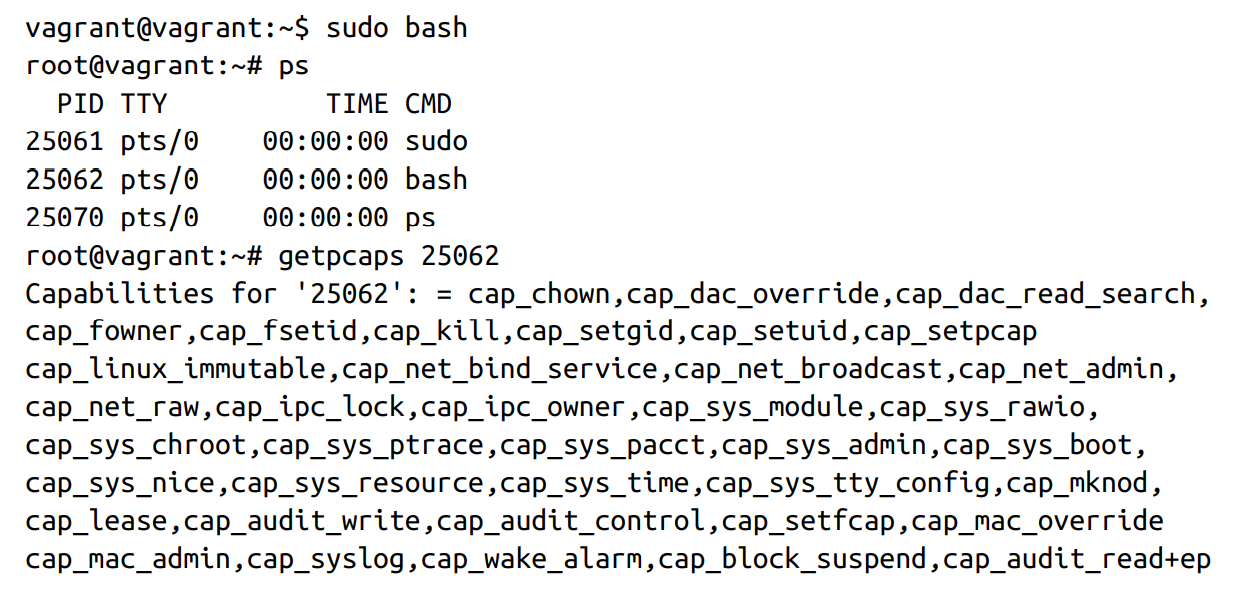
\includegraphics[width=\textwidth, keepaspectratio]{capitoli/os_security/imgs/cap1.png}
\end{figure}

Le capabilities possono anche essere assegnate direttamente ad un file.
Per farlo bisogna utilizzare il comando \verb|setcap <capabilities> filename|
(ovviamente con privilegi di root). Riprendendo l'esempio di prima proviamo ad
assegnare le capabilities necessarie per far funzionare il comando ping.

\begin{figure}[H]
    \centering
    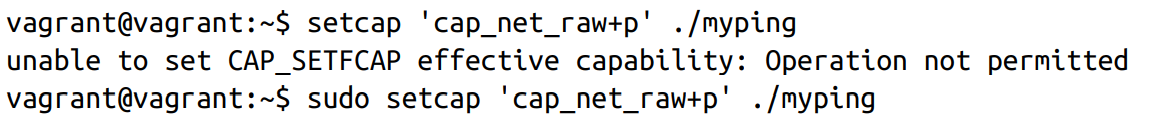
\includegraphics[width=\textwidth, keepaspectratio]{capitoli/os_security/imgs/cap2.png}
\end{figure}

Si può notare che la capabilities  è seguita dal carattere \verb|+p|, essa è un
parametro che va a cambiare le modalità di funzionamento della capability.
Ce ne sono 3 differenti:

\begin{itemize}
    \item \textbf{e} (effective): sta ad indicare che la capability è attiva.
    \item \textbf{p} (permitted): indica che la capability può essere utilizzata.
    \item \textbf{i} (inherited): indica che la capability viene mantenuta
          da un processo figlio
\end{itemize}

Anche utilizzando le capabilities è sempre bene utilizzare il principio del
\textit{least privilege}, ovvero vanno fornite solo le capabilities che sono
strettamente necessaire al funzionamento del programma.

\subsection{Privilege Escalation}

Questo è un tipo di attacco che punta ad estendere i privilegi che si hanno a
disposizione per poter effettuare azioni che non si dovrebbero poter compiere.
Un metodo comune per effettuare questo tipo di attacco è quello di cercare delle
vulnerabilità nel software, un esempio è la \textbf{Struts vulnerability}.